\documentclass{article}
\usepackage[margin=1in]{geometry}
\usepackage[linesnumbered,ruled,vlined]{algorithm2e}
\usepackage{amsfonts}
\usepackage{amsmath}
\usepackage{amssymb}
\usepackage{amsthm}
\usepackage{enumitem}
\usepackage{fancyhdr}
\usepackage{hyperref}
\usepackage{minted}
\usepackage{multicol}
\usepackage{pdfpages}
\usepackage{standalone}
\usepackage[many]{tcolorbox}
\usepackage{tikz-cd}
\usepackage{transparent}
\usepackage{xcolor}
% \tcbuselibrary{minted}

\author{Nathan Solomon}

\newcommand{\fig}[1]{
    \begin{center}
        \includegraphics[width=\textwidth]{#1}
    \end{center}
}

% Math commands
\renewcommand{\d}{\mathrm{d}}
\DeclareMathOperator{\id}{id}
\DeclareMathOperator{\im}{im}
\DeclareMathOperator{\proj}{proj}
\DeclareMathOperator{\Span}{span}
\DeclareMathOperator{\Tr}{Tr}
\DeclareMathOperator{\tr}{tr}
\DeclareMathOperator{\ad}{ad}
\DeclareMathOperator{\ord}{ord}
%%%%%%%%%%%%%%% \DeclareMathOperator{\sgn}{sgn}
\DeclareMathOperator{\Aut}{Aut}
\DeclareMathOperator{\Inn}{Inn}
\DeclareMathOperator{\Out}{Out}
\DeclareMathOperator{\stab}{stab}

\newcommand{\N}{\ensuremath{\mathbb{N}}}
\newcommand{\Z}{\ensuremath{\mathbb{Z}}}
\newcommand{\Q}{\ensuremath{\mathbb{Q}}}
\newcommand{\R}{\ensuremath{\mathbb{R}}}
\newcommand{\C}{\ensuremath{\mathbb{C}}}
\renewcommand{\H}{\ensuremath{\mathbb{H}}}
\newcommand{\F}{\ensuremath{\mathbb{F}}}

\newcommand{\E}{\ensuremath{\mathbb{E}}}
\renewcommand{\P}{\ensuremath{\mathbb{P}}}

\newcommand{\es}{\ensuremath{\varnothing}}
\newcommand{\inv}{\ensuremath{^{-1}}}
\newcommand{\eps}{\ensuremath{\varepsilon}}
\newcommand{\del}{\ensuremath{\partial}}
\renewcommand{\a}{\ensuremath{\alpha}}

\newcommand{\abs}[1]{\ensuremath{\left\lvert #1 \right\rvert}}
\newcommand{\norm}[1]{\ensuremath{\left\lVert #1\right\rVert}}
\newcommand{\mean}[1]{\ensuremath{\left\langle #1 \right\rangle}}
\newcommand{\floor}[1]{\ensuremath{\left\lfloor #1 \right\rfloor}}
\newcommand{\ceil}[1]{\ensuremath{\left\lceil #1 \right\rceil}}
\newcommand{\bra}[1]{\ensuremath{\left\langle #1 \right\rvert}}
\newcommand{\ket}[1]{\ensuremath{\left\lvert #1 \right\rangle}}
\newcommand{\braket}[2]{\ensuremath{\left.\left\langle #1\right\vert #2 \right\rangle}}

\newcommand{\catname}[1]{{\normalfont\textbf{#1}}}

\newcommand{\up}{\ensuremath{\uparrow}}
\newcommand{\down}{\ensuremath{\downarrow}}

% Custom environments
\newtheorem{thm}{Theorem}[section]

\definecolor{probBackgroundColor}{RGB}{250,240,240}
\definecolor{probAccentColor}{RGB}{140,40,0}
\newenvironment{prob}{
    \stepcounter{thm}
    \begin{tcolorbox}[
        boxrule=1pt,
        sharp corners,
        colback=probBackgroundColor,
        colframe=probAccentColor,
        borderline west={4pt}{0pt}{probAccentColor},
        breakable
    ]
    \color{probAccentColor}\textbf{Problem \thethm.} \color{black}
} {
    \end{tcolorbox}
}

\definecolor{exampleBackgroundColor}{RGB}{212,232,246}
\newenvironment{example}{
    \stepcounter{thm}
    \begin{tcolorbox}[
      boxrule=1pt,
      sharp corners,
      colback=exampleBackgroundColor,
      breakable
    ]
    \textbf{Example \thethm.}
} {
    \end{tcolorbox}
}

\definecolor{propBackgroundColor}{RGB}{255,245,220}
\definecolor{propAccentColor}{RGB}{150,100,0}
\newenvironment{prop}{
    \stepcounter{thm}
    \begin{tcolorbox}[
        boxrule=1pt,
        sharp corners,
        colback=propBackgroundColor,
        colframe=propAccentColor,
        breakable
    ]
    \color{propAccentColor}\textbf{Proposition \thethm. }\color{black}
} {
    \end{tcolorbox}
}

\definecolor{thmBackgroundColor}{RGB}{235,225,245}
\definecolor{thmAccentColor}{RGB}{50,0,100}
\renewenvironment{thm}{
    \stepcounter{thm}
    \begin{tcolorbox}[
        boxrule=1pt,
        sharp corners,
        colback=thmBackgroundColor,
        colframe=thmAccentColor,
        breakable
    ]
    \color{thmAccentColor}\textbf{Theorem \thethm. }\color{black}
} {
    \end{tcolorbox}
}

\definecolor{corBackgroundColor}{RGB}{240,250,250}
\definecolor{corAccentColor}{RGB}{50,100,100}
\newenvironment{cor}{
    \stepcounter{thm}
    \begin{tcolorbox}[
        enhanced,
        boxrule=0pt,
        frame hidden,
        sharp corners,
        colback=corBackgroundColor,
        borderline west={4pt}{0pt}{corAccentColor},
        breakable
    ]
    \color{corAccentColor}\textbf{Corollary \thethm. }\color{black}
} {
    \end{tcolorbox}
}

\definecolor{lemBackgroundColor}{RGB}{255,245,235}
\definecolor{lemAccentColor}{RGB}{250,125,0}
\newenvironment{lem}{
    \stepcounter{thm}
    \begin{tcolorbox}[
        enhanced,
        boxrule=0pt,
        frame hidden,
        sharp corners,
        colback=lemBackgroundColor,
        borderline west={4pt}{0pt}{lemAccentColor},
        breakable
    ]
    \color{lemAccentColor}\textbf{Lemma \thethm. }\color{black}
} {
    \end{tcolorbox}
}

\definecolor{proofBackgroundColor}{RGB}{255,255,255}
\definecolor{proofAccentColor}{RGB}{80,80,80}
\renewenvironment{proof}{
    \begin{tcolorbox}[
        enhanced,
        boxrule=1pt,
        sharp corners,
        colback=proofBackgroundColor,
        colframe=proofAccentColor,
        borderline west={4pt}{0pt}{proofAccentColor},
        breakable
    ]
    \color{proofAccentColor}\emph{\textbf{Proof. }}\color{black}
} {
    \qed \end{tcolorbox}
}

\definecolor{noteBackgroundColor}{RGB}{240,250,240}
\definecolor{noteAccentColor}{RGB}{30,130,30}
\newenvironment{note}{
    \begin{tcolorbox}[
        enhanced,
        boxrule=0pt,
        frame hidden,
        sharp corners,
        colback=noteBackgroundColor,
        borderline west={4pt}{0pt}{noteAccentColor},
        breakable
    ]
    \color{noteAccentColor}\textbf{Note. }\color{black}
} {
    \end{tcolorbox}
}


\fancyhf{}
\setlength{\headheight}{24pt}

\date{\today}
\title{Physics 180E Homework \#4}

\begin{document}
\maketitle

\begin{prob}
\end{prob}
Assuming we only have first ionization, the ion saturation current is given by
\[ I_{sat} = n e A \exp \left( - \frac{1}{2} \right)  \sqrt{ \frac{k_B T_e}{M_{ion}}}. \]
The mass of an argon atom is $M_{ion} = 37.2 \si{.GeV/c^2}$. Solving for the plasma density $n$, that becomes
\begin{align*}
\frac{1}{n} &= \frac{eA}{I_{sat}} \exp \left( - \frac{1}{2} \right)  \sqrt{ \frac{k_B T_e}{M_{ion}}} \\
  &= \frac{(1.602 \times 10^{-19} \si{.C})(2\si{.mm})^2}{10^{-4} \si{.A}} \exp \left( - \frac{1}{2} \right)  \sqrt{ \frac{2 \si{.eV}}{3.72 \times 10^{10} \si{.eV/c^2}}} \\
  &= (1.602 \times 10^{-15} \si{.s})(0.002\si{.m})^2 (0.6065) \sqrt{ \frac{2 \cdot (3 \times 10^8 \si{.m/s})^2}{3.72 \times 10^{10}}} \\
  &= (1.602 \times 10^{-15} \si{.s})(4 \times 10^{-6} \si{.m^2}) (0.6065) (3 \times 10^8 \si{m/s}) \sqrt{ \frac{2}{3.72 \times 10^{10}}} \\
  &= (1.602 \times 10^{-15})(4 \times 10^{-6}) (0.6065) (3 \times 10^8) (7.33 \times 10^{-6}) \si{.m^3} \\
  &= 8.55 \times 10^{-18} \si{.m^3} \\
  n &= 1.17 \times 10^{17} \si{.m^{-3}},
\end{align*}
meaning there are $1.17 \times 10^{17}$ argon ions per cubic meter.
\par
The plasma potential is given by the following equation:
\begin{align*}
    V_p &= V_f + \frac{k_B T_e}{2 e} \left( 1 - \log \left( \frac{2 m_e \pi}{M_{ion}} \right) \right) \\
        &= (2\si{.V}) + \frac{2 \si{.eV}}{2 e} \left( 1 - \log \left( \frac{2 \pi (0.511 \si{.MeV/c^2})}{37.2 \si{.GeV/c^2}} \right) \right) \\
        &= (2\si{.V}) + (1 \si{.V}) \cdot \left( 1 - \log \left( 2 \pi (0.511)/37200 \right) \right) \\
        &= (2\si{.V}) + (1 \si{.V}) \cdot \left( 1 - \log (0.0000863) \right) \\
        &= (2\si{.V}) + (1 \si{.V}) \cdot \left( 1 - (-9.36) \right) \\
        &= 12.36 \si{.V}.
\end{align*}

\bigskip
\par
\begin{prob}
\end{prob}
I will assume that the electrons don't collide with neutrals enough to heat the neutral temperature much above room temperature (300 Kelvin). If we assume the cross-sectional area of a neutral argon atom (colliding with an electron) is $\sigma = 10^{-15} \si{.cm^2}=10^{-19} \si{.m^2}$, then the mean free path for electrons is
\begin{align*}
    \ell_{mfp} &= \frac{1}{n \sigma} \\
         &= \frac{k_B T}{p \sigma} \\
         &= \frac{k_B (300\si{.K})}{(1 \si{.mTorr})(10^{-19} \si{.m^2})} \\
         &= \frac{4.14 \times 10^{-21} \si{.J}}{(0.00133 \si{.Pa})(10^{-19} \si{.m^2})} \\
         &= 31.1 \si{.m}.
\end{align*}
The Debye length of the plasma is
\begin{align*}
    \lambda_D &= \sqrt{ \frac{\varepsilon_0 k_B T_e}{e^2 n} } \\
              &= \sqrt{ \frac{\varepsilon_0 (5 \si{.eV})}{e^2 (10^{19} \si{.m^{-3}})}} \\
              &= \sqrt{ \varepsilon_0 (5\si{.V})(10^{-19}\si{.m^3})/e } \\
              &= \sqrt{ (5.526 \times 10^7 \si{.e/V/m}) (5\si{.V})(10^{-19}\si{.m^3})/e } \\
              &= \sqrt{ (5.526 \times 10^7) (5\times 10^{-19}\si{.m^2}) } \\
              &= 5.26 \si{.\mu m}.
\end{align*}
The mean free path of electrons is much, much larger than the Debye length, meaning collisions don't occur much within the sheath around the Langmuir probe. In fact, since the mean free path is very large, we can think of collisions as being fairly rare, which is why the neutrals and the electrons are allowed to have different temperatures -- if they collided very often, they would exchange heat and approach thermal equilibrium.

\bigskip
\par
\begin{prob}
\end{prob}
Here is the IV curve for a single Langmuir sweep (before and after filtering):
\begin{center}
    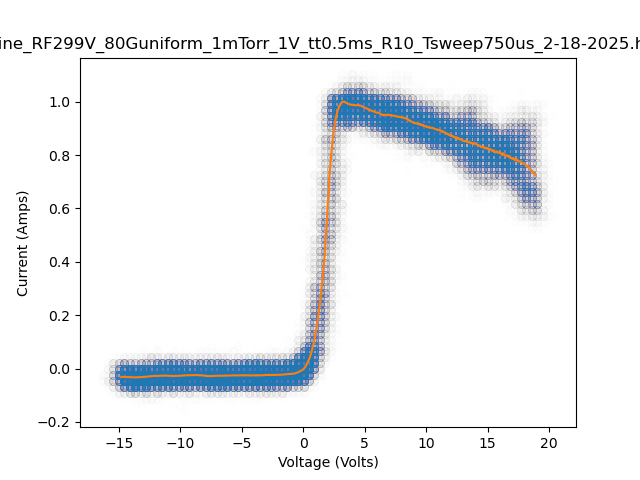
\includegraphics[width=\textwidth]{Figure_1.png}
\end{center}
I then took the derivative of that data and fitted the result to an equation of the form
\[ \frac{\partial I_{probe}}{\partial \phi} = n e^2 A \sqrt{ \frac{1}{2 \pi k_B m_e T_e}} \exp \left( - \frac{e (\phi-V_0)}{2 k_B T_e} \right) \]
in order to extract the electron temperature ($T_e$), the plasma potential ($V_0$), and the electron density ($n$).
\begin{center}
    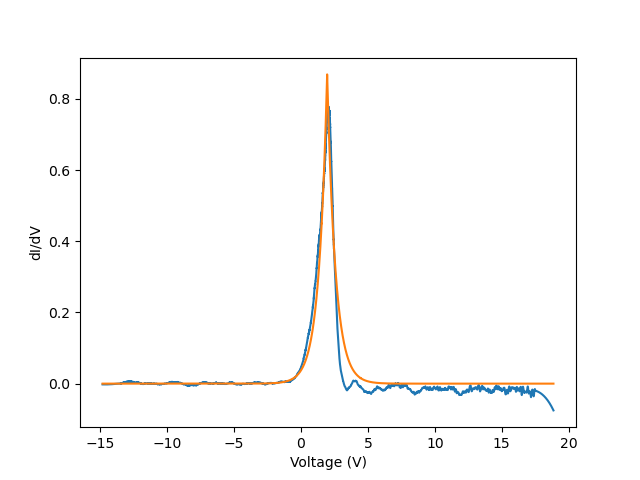
\includegraphics[width=\textwidth]{Figure_2.png}
\end{center}

\begin{itemize}
    \item Electron temperature: $0.31045 \si{.eV}$
    \item Plasma potential: $1.9565 \si{.V}$
    \item Electron density: $4.5136 \times 10^{18} \si{.m^{-3}}$
\end{itemize}

\bigskip
\par
\begin{prob}
\end{prob}
\begin{enumerate}[label=(\alph*)]
    \item Yes, they look like roughly the right order of magnitude.
    \item The first ionization energy of argon is $15.76 \si{.eV}$, which is much larger than the electron temperature I found. That means that the temperature is way too small for ``bulk ionization". For thermal collisions between electrons and neutrals to ionize a non-negligible proportion of the argon atoms, the electron temperature would have to bean close to the ionization energy of argon.
\end{enumerate}


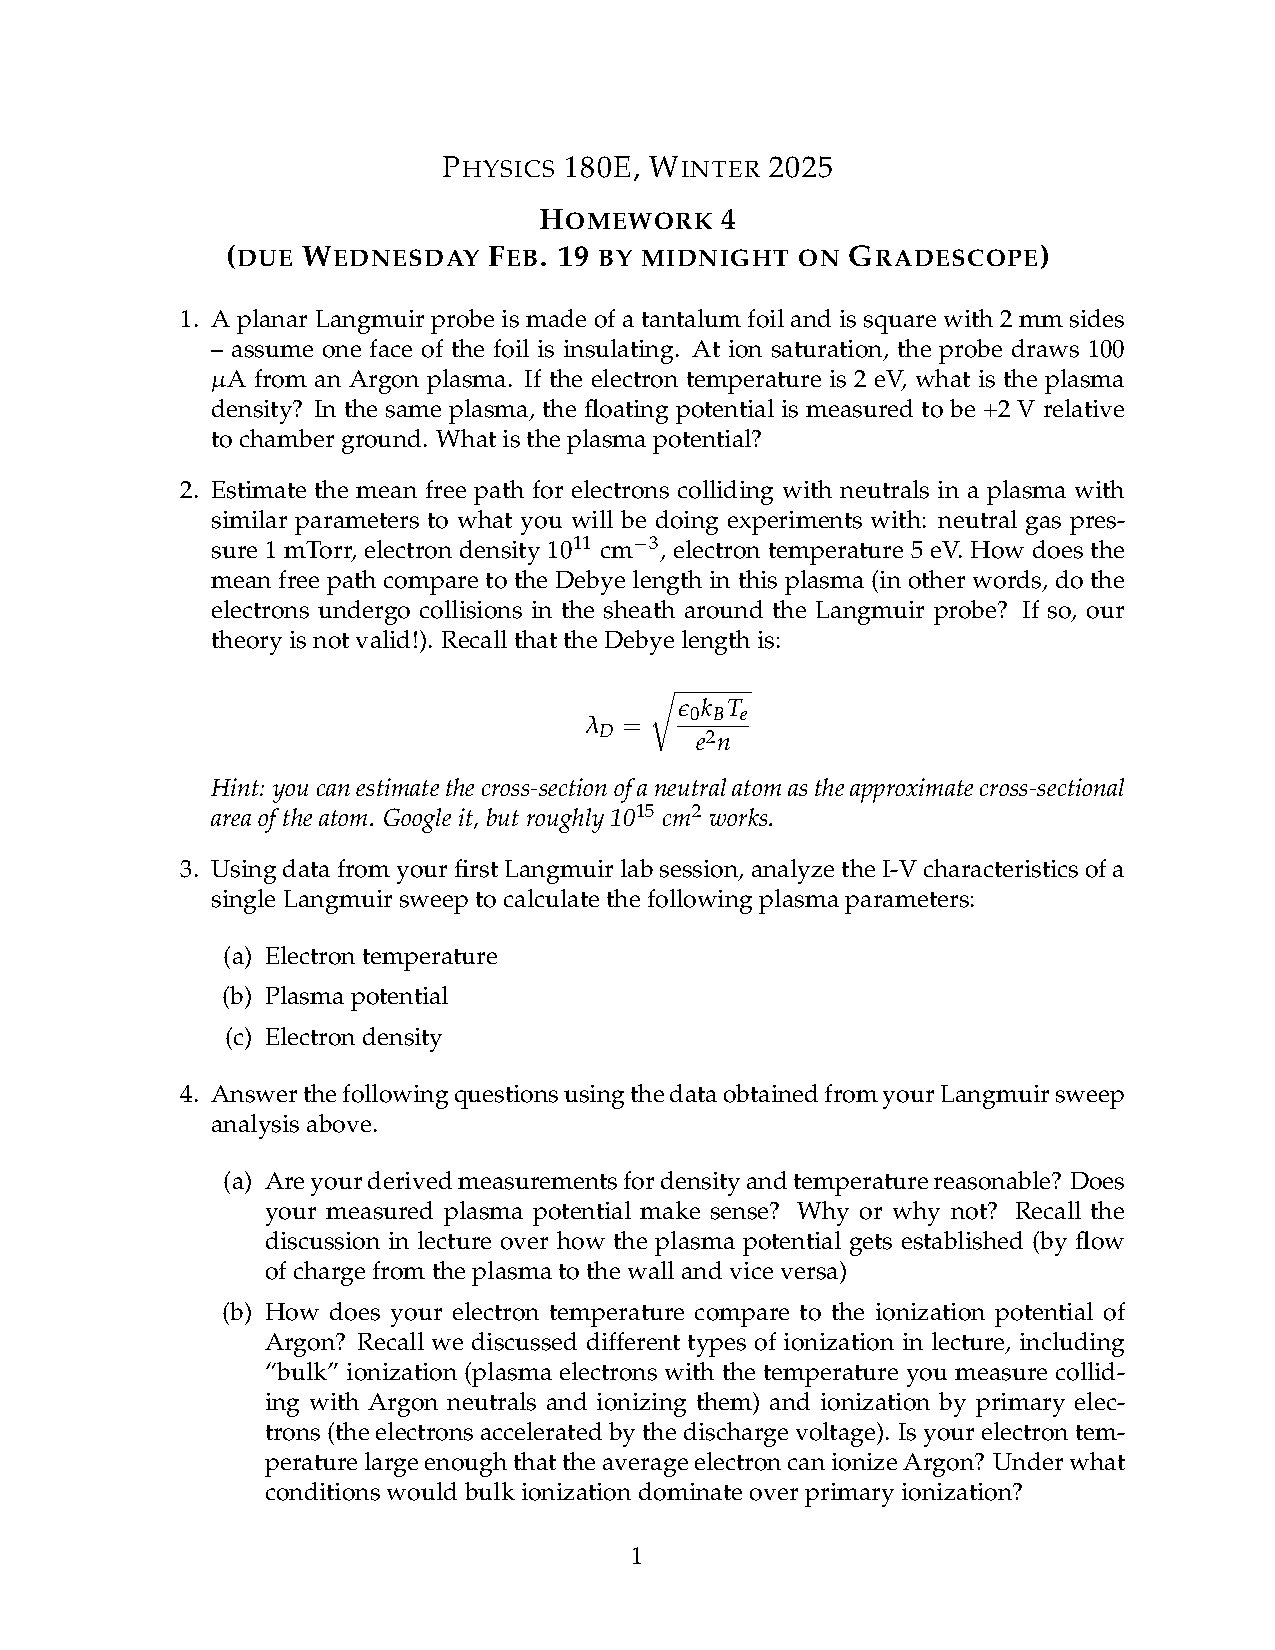
\includepdf[pages=-]{assignment.pdf}

\end{document}
